% Options for packages loaded elsewhere
% Options for packages loaded elsewhere
\PassOptionsToPackage{unicode}{hyperref}
\PassOptionsToPackage{hyphens}{url}
\PassOptionsToPackage{dvipsnames,svgnames,x11names}{xcolor}
%
\documentclass[
]{article}
\usepackage{xcolor}
\usepackage[margin=1in]{geometry}
\usepackage{amsmath,amssymb}
\setcounter{secnumdepth}{-\maxdimen} % remove section numbering
\usepackage{iftex}
\ifPDFTeX
  \usepackage[T1]{fontenc}
  \usepackage[utf8]{inputenc}
  \usepackage{textcomp} % provide euro and other symbols
\else % if luatex or xetex
  \usepackage{unicode-math} % this also loads fontspec
  \defaultfontfeatures{Scale=MatchLowercase}
  \defaultfontfeatures[\rmfamily]{Ligatures=TeX,Scale=1}
\fi
\usepackage{lmodern}
\ifPDFTeX\else
  % xetex/luatex font selection
\fi
% Use upquote if available, for straight quotes in verbatim environments
\IfFileExists{upquote.sty}{\usepackage{upquote}}{}
\IfFileExists{microtype.sty}{% use microtype if available
  \usepackage[]{microtype}
  \UseMicrotypeSet[protrusion]{basicmath} % disable protrusion for tt fonts
}{}
\makeatletter
\@ifundefined{KOMAClassName}{% if non-KOMA class
  \IfFileExists{parskip.sty}{%
    \usepackage{parskip}
  }{% else
    \setlength{\parindent}{0pt}
    \setlength{\parskip}{6pt plus 2pt minus 1pt}}
}{% if KOMA class
  \KOMAoptions{parskip=half}}
\makeatother
% Make \paragraph and \subparagraph free-standing
\makeatletter
\ifx\paragraph\undefined\else
  \let\oldparagraph\paragraph
  \renewcommand{\paragraph}{
    \@ifstar
      \xxxParagraphStar
      \xxxParagraphNoStar
  }
  \newcommand{\xxxParagraphStar}[1]{\oldparagraph*{#1}\mbox{}}
  \newcommand{\xxxParagraphNoStar}[1]{\oldparagraph{#1}\mbox{}}
\fi
\ifx\subparagraph\undefined\else
  \let\oldsubparagraph\subparagraph
  \renewcommand{\subparagraph}{
    \@ifstar
      \xxxSubParagraphStar
      \xxxSubParagraphNoStar
  }
  \newcommand{\xxxSubParagraphStar}[1]{\oldsubparagraph*{#1}\mbox{}}
  \newcommand{\xxxSubParagraphNoStar}[1]{\oldsubparagraph{#1}\mbox{}}
\fi
\makeatother


\usepackage{longtable,booktabs,array}
\newcounter{none} % for unnumbered tables
\usepackage{calc} % for calculating minipage widths
% Correct order of tables after \paragraph or \subparagraph
\usepackage{etoolbox}
\makeatletter
\patchcmd\longtable{\par}{\if@noskipsec\mbox{}\fi\par}{}{}
\makeatother
% Allow footnotes in longtable head/foot
\IfFileExists{footnotehyper.sty}{\usepackage{footnotehyper}}{\usepackage{footnote}}
\makesavenoteenv{longtable}
\usepackage{graphicx}
\makeatletter
\newsavebox\pandoc@box
\newcommand*\pandocbounded[1]{% scales image to fit in text height/width
  \sbox\pandoc@box{#1}%
  \Gscale@div\@tempa{\textheight}{\dimexpr\ht\pandoc@box+\dp\pandoc@box\relax}%
  \Gscale@div\@tempb{\linewidth}{\wd\pandoc@box}%
  \ifdim\@tempb\p@<\@tempa\p@\let\@tempa\@tempb\fi% select the smaller of both
  \ifdim\@tempa\p@<\p@\scalebox{\@tempa}{\usebox\pandoc@box}%
  \else\usebox{\pandoc@box}%
  \fi%
}
% Set default figure placement to htbp
\def\fps@figure{htbp}
\makeatother





\setlength{\emergencystretch}{3em} % prevent overfull lines

\providecommand{\tightlist}{%
  \setlength{\itemsep}{0pt}\setlength{\parskip}{0pt}}



 


\makeatletter
\@ifpackageloaded{tcolorbox}{}{\usepackage[skins,breakable]{tcolorbox}}
\@ifpackageloaded{fontawesome5}{}{\usepackage{fontawesome5}}
\definecolor{quarto-callout-color}{HTML}{909090}
\definecolor{quarto-callout-note-color}{HTML}{0758E5}
\definecolor{quarto-callout-important-color}{HTML}{CC1914}
\definecolor{quarto-callout-warning-color}{HTML}{EB9113}
\definecolor{quarto-callout-tip-color}{HTML}{00A047}
\definecolor{quarto-callout-caution-color}{HTML}{FC5300}
\definecolor{quarto-callout-color-frame}{HTML}{acacac}
\definecolor{quarto-callout-note-color-frame}{HTML}{4582ec}
\definecolor{quarto-callout-important-color-frame}{HTML}{d9534f}
\definecolor{quarto-callout-warning-color-frame}{HTML}{f0ad4e}
\definecolor{quarto-callout-tip-color-frame}{HTML}{02b875}
\definecolor{quarto-callout-caution-color-frame}{HTML}{fd7e14}
\makeatother
\makeatletter
\@ifpackageloaded{caption}{}{\usepackage{caption}}
\AtBeginDocument{%
\ifdefined\contentsname
  \renewcommand*\contentsname{Table of contents}
\else
  \newcommand\contentsname{Table of contents}
\fi
\ifdefined\listfigurename
  \renewcommand*\listfigurename{List of Figures}
\else
  \newcommand\listfigurename{List of Figures}
\fi
\ifdefined\listtablename
  \renewcommand*\listtablename{List of Tables}
\else
  \newcommand\listtablename{List of Tables}
\fi
\ifdefined\figurename
  \renewcommand*\figurename{Figure}
\else
  \newcommand\figurename{Figure}
\fi
\ifdefined\tablename
  \renewcommand*\tablename{Table}
\else
  \newcommand\tablename{Table}
\fi
}
\@ifpackageloaded{float}{}{\usepackage{float}}
\floatstyle{ruled}
\@ifundefined{c@chapter}{\newfloat{codelisting}{h}{lop}}{\newfloat{codelisting}{h}{lop}[chapter]}
\floatname{codelisting}{Listing}
\newcommand*\listoflistings{\listof{codelisting}{List of Listings}}
\makeatother
\makeatletter
\makeatother
\makeatletter
\@ifpackageloaded{caption}{}{\usepackage{caption}}
\@ifpackageloaded{subcaption}{}{\usepackage{subcaption}}
\makeatother
\usepackage{bookmark}
\IfFileExists{xurl.sty}{\usepackage{xurl}}{} % add URL line breaks if available
\urlstyle{same}
\hypersetup{
  pdftitle={Looking for the log-multiplication trick inside GPT-2},
  pdfauthor={hl},
  colorlinks=true,
  linkcolor={blue},
  filecolor={Maroon},
  citecolor={Blue},
  urlcolor={Blue},
  pdfcreator={LaTeX via pandoc}}


\title{Looking for the log-multiplication trick inside GPT-2}
\usepackage{etoolbox}
\makeatletter
\providecommand{\subtitle}[1]{% add subtitle to \maketitle
  \apptocmd{\@title}{\par {\large #1 \par}}{}{}
}
\makeatother
\subtitle{A mechanistic-interpretability study of how a small language
model represents numbers, and whether it secretly knows that
\(a \cdot b = 2^{\log_2 a + \log_2 b}\).}
\author{hl}
\date{2026-05-12}
\begin{document}
\maketitle
\begin{abstract}
Multiplication has a famous shortcut: replace it with logarithm +
addition + exponentiation. This post asks whether GPT-2 small (124M
parameters) implements that shortcut internally. Using linear probes and
activation patching, I find that (1) the token embedding represents
number magnitude on a roughly logarithmic axis at \(R^2 = 0.95\), with
separate axes for parity and last digit but not for arbitrary
number-theoretic properties; (2) perturbing the embedding's log axis has
direction-specific causal effect on next-token predictions, while random
perturbations of equal magnitude do not; and (3) GPT-2 genuinely
computes \(\log_2(a \cdot b)\) in its residual stream at the \texttt{=}
position, but on a \emph{different} direction than the one used to read
the operands. The \(\log \to \mathrm{sum} \to \exp\) machine is
mechanistically present in the model, even though the LM head's strong
frequency prior prevents the circuit from producing correct arithmetic
behaviour.
\end{abstract}

\renewcommand*\contentsname{Table of contents}
{
\setcounter{tocdepth}{3}
\tableofcontents
}

Multiplication is hard work, but it has a famous shortcut. For three
centuries, before the pocket calculator, scientists and engineers
carried slide rules --- physical implementations of the identity

\begin{equation}\protect\phantomsection\label{eq-shortcut}{
a \cdot b = 2^{\log_2 a + \log_2 b}
}\end{equation}

Instead of multiplying two numbers, you look up their logarithms, add
the logs (which is easy), and look up the exponential of the sum. The
whole trick rests on a different geometry of number: position by log
magnitude, not by raw magnitude.

A natural question, then: does a neural network ever discover this
shortcut? If you train a small model to multiply, does it secretly learn
the slide rule? The longer plan in \texttt{experiment1.md} proposes
training a fresh tiny Transformer from scratch under capacity pressure
and then dissecting it. This post is the parallel question: \textbf{is
the shortcut already sitting inside an existing small language model?} I
went looking, in GPT-2 small, with linear probes and activation
patching.

\begin{tcolorbox}[enhanced jigsaw, arc=.35mm, bottomrule=.15mm, bottomtitle=1mm, breakable, colback=white, colbacktitle=quarto-callout-note-color!10!white, colframe=quarto-callout-note-color-frame, coltitle=black, left=2mm, leftrule=.75mm, opacityback=0, opacitybacktitle=0.6, rightrule=.15mm, title=\textcolor{quarto-callout-note-color}{\faInfo}\hspace{0.5em}{Summary}, titlerule=0mm, toprule=.15mm, toptitle=1mm]

GPT-2 has the \emph{substrate} of the shortcut. Its token embeddings
represent number magnitude on a roughly logarithmic axis (\(R^2 = 0.95\)
at layer 0). That axis has structured, direction-specific causal effect
on the model's next-token predictions in multiplication prompts. And the
model genuinely computes \(\log_2(a \cdot b)\) in its residual stream
right before the LM head --- a fresh probe at the \texttt{=} position
predicts the answer's log at \(R^2 = 0.989\). The whole
\(\log \to \mathrm{sum} \to \exp\) machine is wired up. What's missing
for behavioural success is not the circuit but the LM head's willingness
to act on it: GPT-2's strong frequency prior for small numbers dominates
the output distribution, so even though the machine exists, GPT-2 can't
actually multiply \(5 \times 9\) and get \(45\).

\end{tcolorbox}

There's also a methodological lesson hidden in the story. I almost
concluded ``no circuit'' after the input-side probe came up flat at the
\texttt{=} position. Training a fresh probe in the right place rescued
the result. Probes are cheap. Don't assume the same direction does
double duty.

\subsection{A toy model, as a yardstick}\label{sec-toy-model}

Before touching any real model, I built a normative toy to make the
cost-pressure hypothesis quantitative. Two paths can compute
\(z = a \cdot b\):

\begin{itemize}
\tightlist
\item
  \textbf{Direct multiplication}, cost
  \(c_{\mathrm{mul}}(a, b) = \log_2(a) \cdot \log_2(b)\) --- the bit
  \(\times\) bit schoolbook work. Multiplying \(2 \times 2\) is one bit
  times one bit (cheap); \(1024 \times 512\) is ten bits times nine
  (expensive).
\item
  \textbf{The log-sum-exp shortcut}, cost \(c_{\mathrm{short}} = 6\) ---
  a small constant for one logarithm lookup, one addition, one
  exponential lookup.
\end{itemize}

A small neural gate reads \((\log_2 a, \log_2 b)\) and produces a
probability \(p \in [0, 1]\) of taking the shortcut. The expected total
cost at penalty weight \(\lambda\) is

\begin{equation}\protect\phantomsection\label{eq-cost}{
C(p, a, b, \lambda) = (1-p)\cdot \lambda \cdot c_{\mathrm{mul}}(a, b) + p \cdot c_{\mathrm{short}}.
}\end{equation}

Sweep \(\lambda\). At each value, retrain the gate to minimise expected
cost. Plot the average probability of using the shortcut.

The curve does the expected thing --- a smooth sigmoid from ``always
direct'' to ``almost always shortcut'' --- but the interesting part is
the geometry. Because the cost of direct multiplication depends on
\((a, b)\), different pairs cross over at different \(\lambda\). Hard
multiplications (large \(a \times b\)) switch first, easy ones (small
\(a \times b\)) hold out longer, and trivial ones (those containing
\(1\)) never switch --- \(\log_2(1) = 0\) makes direct multiplication
genuinely free for them, so no penalty can dislodge the direct path.

\begin{figure}

\centering{

\pandocbounded{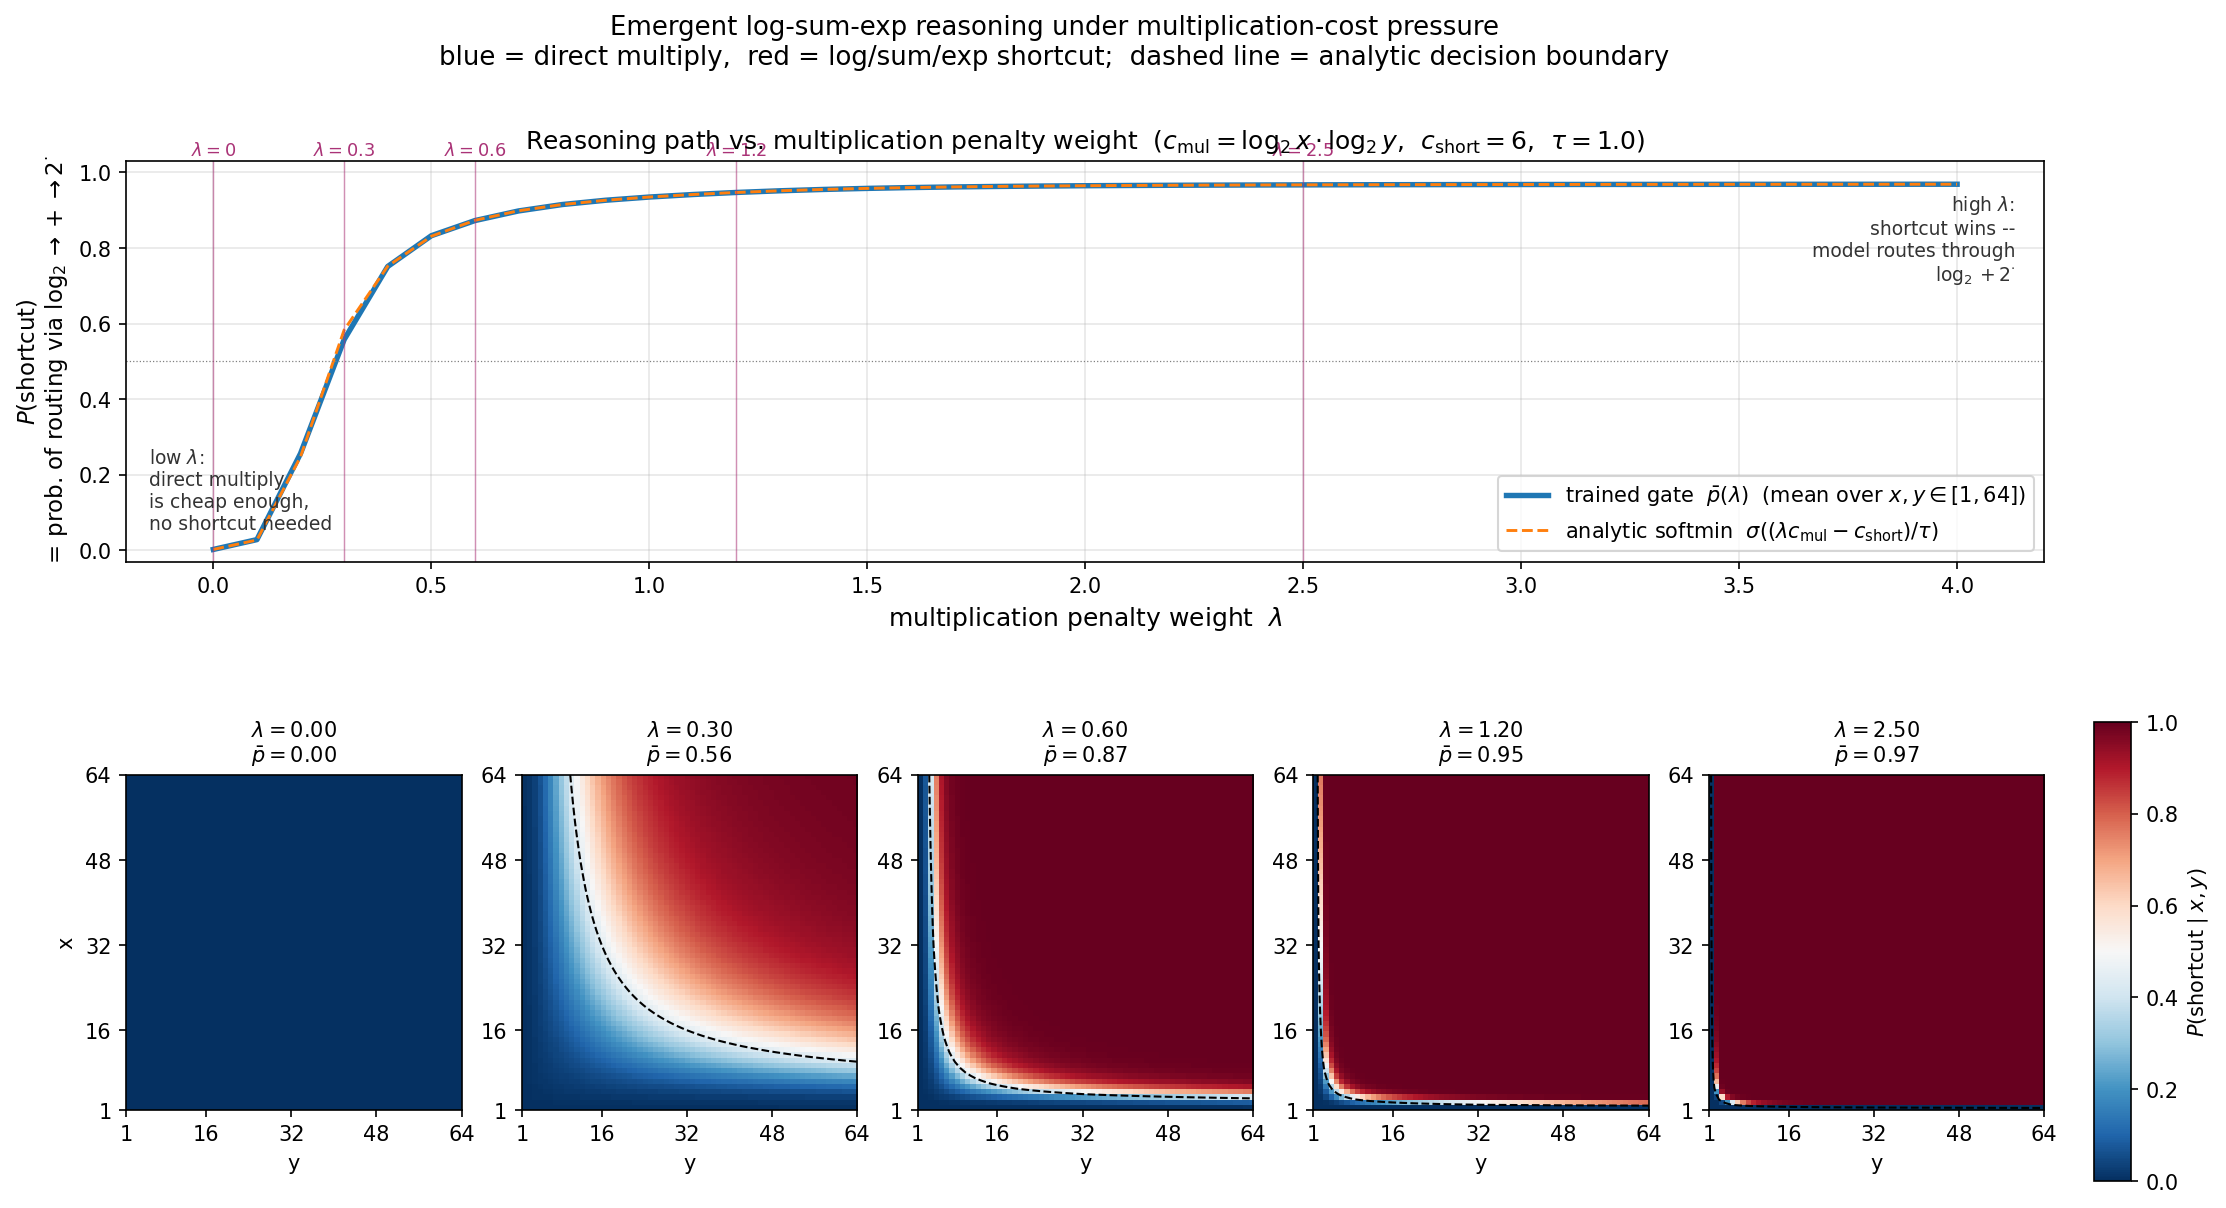
\includegraphics[keepaspectratio]{./reasoning_path_vs_penalty.png}}

}

\caption{\label{fig-toy-routing}Toy soft-routing model. \textbf{Top:}
\(P(\mathrm{shortcut})\) averaged over \((a,b) \in [1,64]^2\) vs the
multiplication penalty weight \(\lambda\). The trained gate (blue)
matches the analytical softmin baseline (orange). \textbf{Bottom:}
per-pair gate at five \(\lambda\) snapshots; the decision boundary
sweeps from upper-right to lower-left as hard multiplications switch
first.}

\end{figure}%

This isn't itself a finding. It's a yardstick. It tells you what an
idealised cost-cutter \emph{should} do under the difficulty function
\(\log_2(a) \cdot \log_2(b)\). The empirical question is whether GPT-2
--- a real model trained on text, not on a multiplication objective ---
shows even a faint trace of this geometry.

\subsection{How GPT-2 represents numbers}\label{sec-embedding-probe}

To check what GPT-2 stores about integers, I fed it the numbers 2
through 1023 one at a time, formatted as \texttt{"\ 5"},
\texttt{"\ 17"}, \texttt{"\ 1024"} and so on (many are single BPE
tokens; multi-token cases use the final position). At every layer I
extracted the residual stream --- the model's internal scratchpad ---
and asked: given the scratchpad, can I predict \(\log_2(x)\) with linear
regression?

\textbf{At the embedding layer --- the raw token embedding, before any
transformer block has run --- \(\log_2(x)\) is decodable at
\(R^2 = 0.95\).} Raw \(x\) is also decodable, but worse, at
\(R^2 = 0.77\). Shuffled labels (a noise control) give
\(R^2 \approx 0\). So the embedding seems to encode magnitude more as
the logarithm than as the number itself.

To make sure the axis is really log-shaped rather than just ``some
monotone function of \(x\)'', I swept the power-law family \(x^\alpha\).
Decodability peaks right around \(\alpha = 0\) (the log limit). If GPT-2
stored linear magnitude the peak would be at \(\alpha = 1\). It isn't
--- it's clearly on the log side.

What's more surprising is what \emph{else} the embedding stores.
\textbf{Parity} --- whether \(x\) is even or odd --- is decodable at
\(R^2 = 0.94\). \textbf{Last digit} (\(x \bmod 10\)) is decodable at
\(R^2 = 0.92\). GPT-2 has noticed, just from reading text, that
\texttt{"\ 5"}, \texttt{"\ 15"}, \texttt{"\ 25"} all share the feature
of ending in \texttt{5}, and has placed those embeddings on a common
axis. But ask the same probe for \texttt{"is\ x\ divisible\ by\ 7?"} and
the \(R^2\) is essentially zero. Same for \texttt{"is\ x\ prime?"}.

So the embedding has structure for the things a careful reader of
natural language might track --- size, parity, last digit --- and
ignores number-theory properties that show up too rarely in text to
matter. That's a small thing, but it tells you what kind of
representation GPT-2 has built. It's the representation of a literate
generalist, not a careful arithmetician.

\begin{figure}

\centering{

\pandocbounded{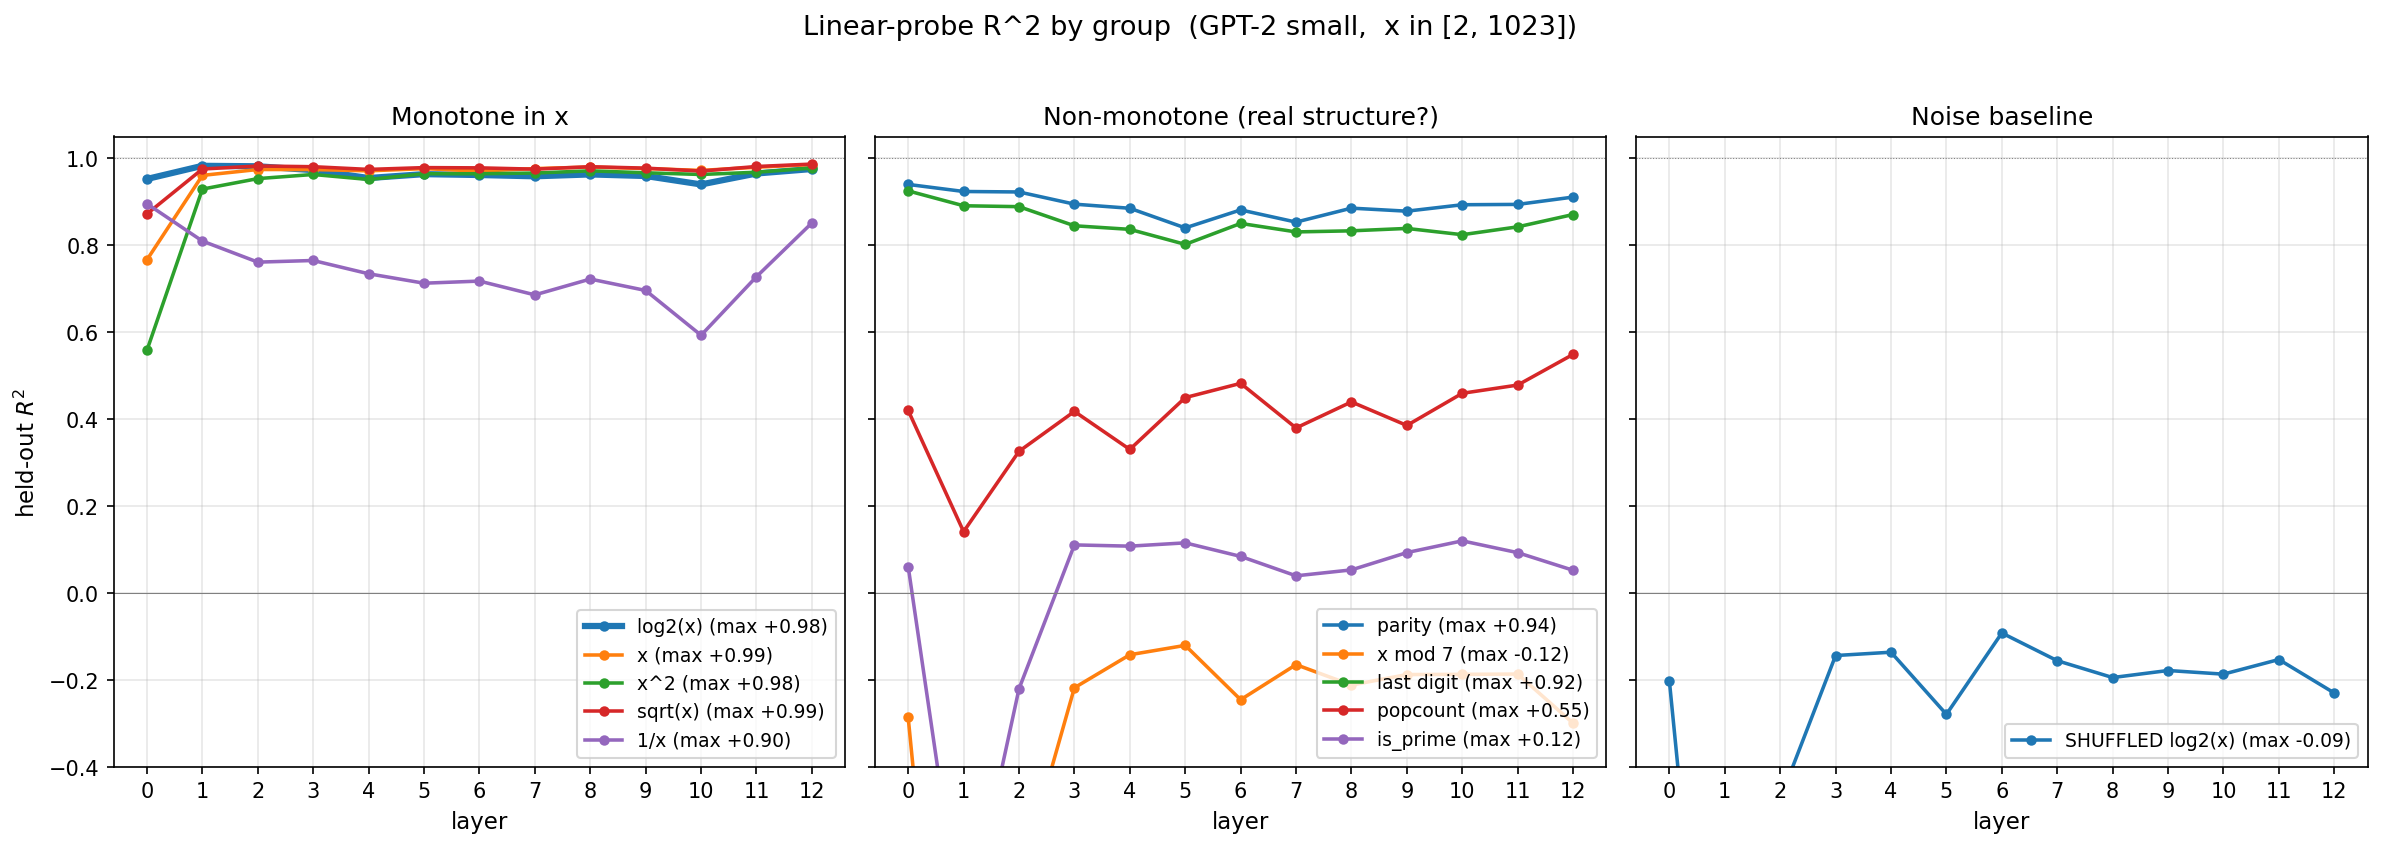
\includegraphics[keepaspectratio]{./probe_gpt2_controls.png}}

}

\caption{\label{fig-controls}Linear-probe \(R^2\) at each layer for
monotone targets (\(\log_2 x\), \(x\), \(x^2\), \(\sqrt{x}\), \(1/x\)),
non-monotone targets (parity, \(x \bmod 7\), last digit, popcount,
is\_prime), and a noise baseline (shuffled \(\log_2 x\)). The log axis,
parity, and last digit are all decodable at the embedding.
Number-theoretic properties and the shuffle control are at chance.}

\end{figure}%

\subsection{Does the model use the log axis when it
multiplies?}\label{sec-causal-patching}

Linear decodability is correlational. To test causality I ran activation
patching at the operand token.

Here's the experiment. Take a prompt like \texttt{"\ 5\ *\ 9\ ="}. The
model processes it normally. At the position where \texttt{"\ 5"} sits,
the embedding's projection onto the probe direction \(w\) reads
\(\log_2(5) \approx 2.3\). I add a rank-1 vector along \(w\) so that
projection now reads \(\log_2(2) = 1\) --- \emph{everything else} about
the embedding is left unchanged. Then I let the model run through all 12
transformer blocks and the LM head, and ask: which numeric token did the
next-token distribution shift toward?

The result: for \texttt{"\ 5\ *\ 9\ ="}, patching
\(\log_2(5) \to \log_2(2)\) makes the logit for \texttt{"\ 18"} (=
\(2 \cdot 9\)) rise \emph{above} the logit for \texttt{"\ 45"} (=
\(5 \cdot 9\)). The model has been talked into preferring the patched
product. Patching toward \(4\) makes \texttt{"\ 36"} win. Patching
toward \(5\) does nothing, as it should. And --- the critical control
--- patching along five different \emph{random} directions of equal
magnitude to \(w\) gives logit shifts indistinguishable from zero. So
the effect is specific to the probe direction, not a generic
perturbation.

There is one wrinkle. Patching \emph{down} (toward smaller numbers)
works cleanly. Patching \emph{up} (toward larger numbers) only partly
works --- the model's preference for the patched product saturates and
then reverses. The most plausible explanation is that the LM head
carries a strong frequency prior favouring small, common numbers in
text, and a fixed-size patch is enough to push preference toward smaller
numbers (with the prior) but not enough to push it toward larger numbers
(against the prior). Either way, the effect on the smaller side is
robust and direction-specific.

\begin{figure}

\centering{

\pandocbounded{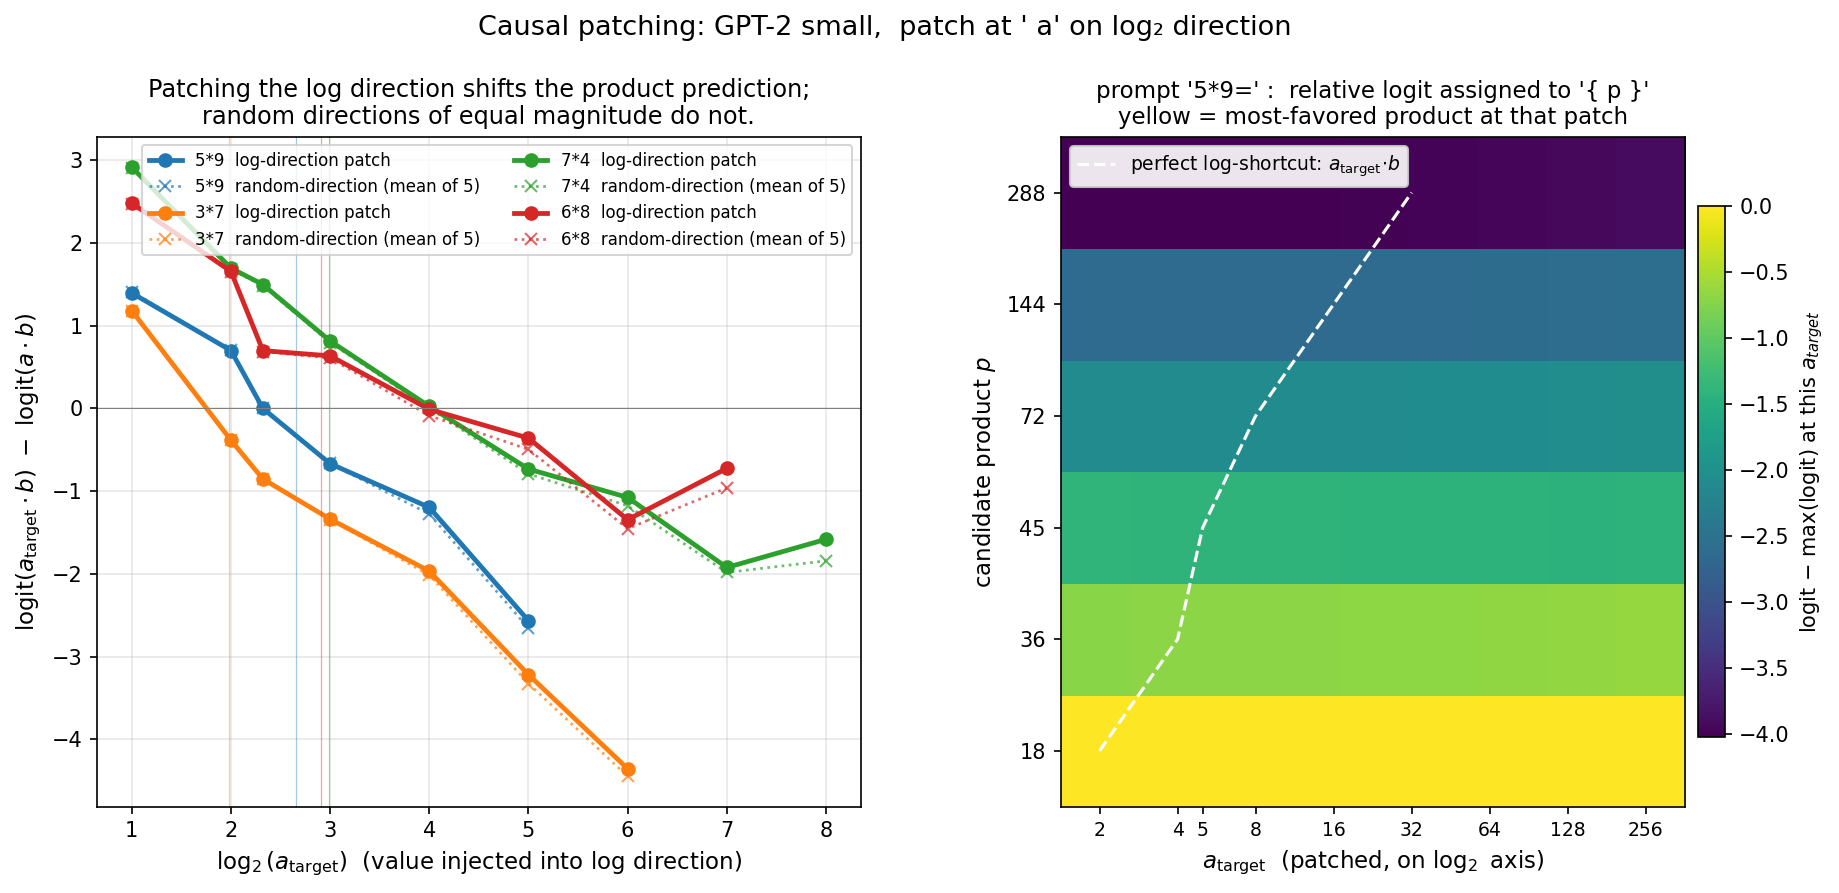
\includegraphics[keepaspectratio]{./probe_gpt2_patching.png}}

}

\caption{\label{fig-patching}Causal patching at the operand.
\textbf{Left:} change in relative logit,
\(\mathrm{logit}(a_{\mathrm{target}} \cdot b) - \mathrm{logit}(a \cdot b)\),
as we patch the log direction at the \texttt{a} position. Solid lines
are the log direction; dotted lines are random directions of the same
norm. \textbf{Right:} heatmap of relative logits assigned to candidate
products for the prompt \texttt{"\ 5\ *\ 9\ ="}. The yellow
most-favoured-product stripe follows the perfect-log-shortcut line
\(p = a_{\mathrm{target}} \cdot b\) for downward patches, then sticks at
\(45\) as we patch toward larger numbers.}

\end{figure}%

\subsection{What's in the LM head?}\label{sec-lm-head}

The LM head --- the matrix that turns the final residual stream into
next-token logits --- has a row for every token. For numeric tokens,
what's in those rows?

\begin{tcolorbox}[enhanced jigsaw, arc=.35mm, bottomrule=.15mm, bottomtitle=1mm, breakable, colback=white, colbacktitle=quarto-callout-warning-color!10!white, colframe=quarto-callout-warning-color-frame, coltitle=black, left=2mm, leftrule=.75mm, opacityback=0, opacitybacktitle=0.6, rightrule=.15mm, title=\textcolor{quarto-callout-warning-color}{\faExclamationTriangle}\hspace{0.5em}{Architectural caveat}, titlerule=0mm, toprule=.15mm, toptitle=1mm]

GPT-2 ties its LM head to the input embedding, so each numeric token's
row is literally the same vector as \(\mathrm{wte}(``\!\!\!\!\!~n")\).
This means the LM head automatically aligns with whatever directions the
embedding aligns with. The interesting question is therefore not
\emph{whether} the LM-head row aligns with the log axis (it does, by
construction), but \emph{how much}. An untied model (Llama, Pythia)
would give a cleaner test.

\end{tcolorbox}

I measured this by projecting each numeric token's LM-head row onto the
unit log direction and asking what fraction of the row's squared norm
sits there. The answer is \textbf{3.6\% on average}. That sounds small,
but a random direction in 768-dimensional space would only capture about
\(1/d = 1/768 \approx 0.13\%\). So the log axis is about
\textbf{28\(\times\) the random baseline} --- a big feature compared to
noise, but a small slice of each row's total content. Parity and
last-digit are above baseline too (about 4\(\times\) random) but
smaller. The remaining roughly 96\% of each row lives on directions I
haven't named, presumably encoding things like ``this is a number'',
``this is a small common number'', and token-specific idiosyncrasies.

The log axis is the largest \emph{identified} feature in the LM head's
numeric rows. It is not the whole row.

\begin{figure}

\centering{

\pandocbounded{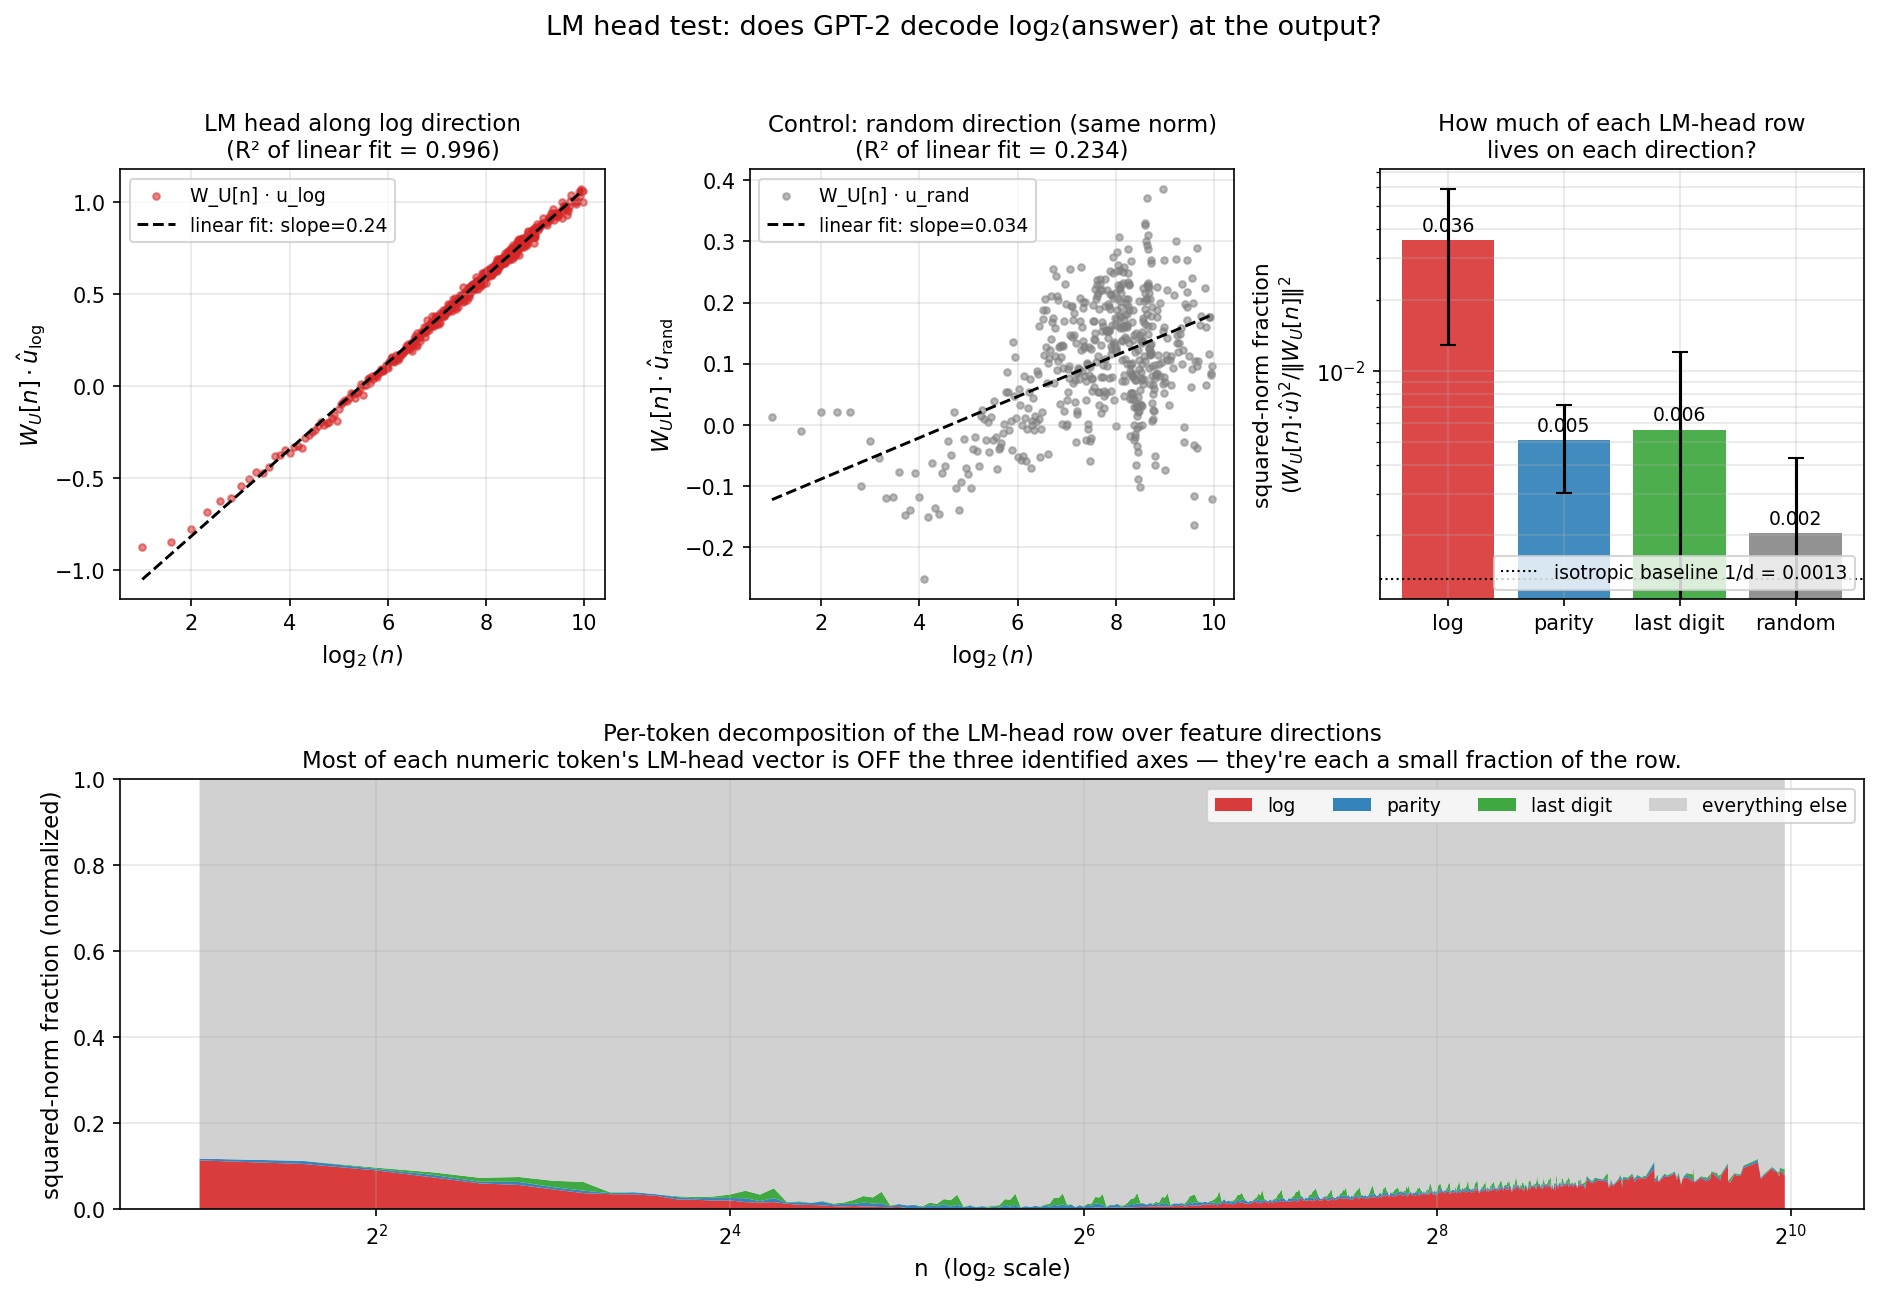
\includegraphics[keepaspectratio]{./probe_gpt2_lmhead.png}}

}

\caption{\label{fig-lmhead}Decomposition of each numeric token's LM-head
row along three identified directions (log, parity, last digit) versus a
same-norm random direction. The log axis captures 3.6\% of each row's
squared norm on average, \textasciitilde28\(\times\) the isotropic
baseline of \(1/d = 0.13\%\). Bottom panel: per-token stacked
composition; the grey ``everything else'' --- directions we haven't
named --- dominates every numeric token's row.}

\end{figure}%

\subsection{Does the model actually compute log(a ·
b)?}\label{sec-pipeline}

This is the test I most wanted to run.

If the model does the slide-rule trick --- adds the operand logs and
then exponentiates at the end --- then at the position of the \texttt{=}
sign, the residual stream right before the LM head should be carrying
\(\log_2(a \cdot b)\). Specifically, the operand-side log direction
\(w\) ought to read off this value.

I checked. For \texttt{"\ 5\ *\ 9\ ="}, the operand-side probe at
\texttt{=} reads off \textbf{10.76} --- not \(\log_2(45) \approx 5.49\).
For \texttt{"\ 3\ *\ 7\ ="} it reads \textbf{11.17}, not
\(\log_2(21) \approx 4.39\). Across nine different prompts, the readout
is essentially flat. The \(R^2\) of ``what the operand-axis probe reads
at \texttt{=}'' against ``the true \(\log_2(a \cdot b)\)'' is
\textbf{0.011} --- no signal.

My first reaction was: well, the circuit isn't there. The shortcut
exists on the input side and in the head's row geometry, but the model
isn't actually wiring them together.

Then it occurred to me: maybe the model uses a \emph{different}
direction at the \texttt{=} position to write down the answer's log than
the one it uses to read the operands' logs. There's no architectural
reason those have to be the same vector --- the model can translate
between representations as it computes. So I trained a fresh ridge probe
directly on the residual at \texttt{=}, against \(\log_2(a \cdot b)\)
for several hundred random \((a, b)\) pairs.

\begin{tcolorbox}[enhanced jigsaw, arc=.35mm, bottomrule=.15mm, bottomtitle=1mm, breakable, colback=white, colbacktitle=quarto-callout-important-color!10!white, colframe=quarto-callout-important-color-frame, coltitle=black, left=2mm, leftrule=.75mm, opacityback=0, opacitybacktitle=0.6, rightrule=.15mm, title=\textcolor{quarto-callout-important-color}{\faExclamation}\hspace{0.5em}{The key result}, titlerule=0mm, toprule=.15mm, toptitle=1mm]

The new probe predicts the answer's log at \(R^2 = 0.989\) on held-out
\((a, b)\) pairs. The model has computed \(\log_2(a \cdot b)\). It's
there. It's almost perfectly linearly decodable from the residual stream
right before the LM head. I had simply been looking on the wrong axis.

\end{tcolorbox}

So the picture is this. The operands' logs are written down on one axis
at the input layer. Somewhere in the middle layers --- I haven't pinned
down where --- the model adds them and rewrites the result on a
\emph{different} axis at the \texttt{=} position. The LM head then reads
that second axis when deciding what number comes next. The whole
\(\log \to \mathrm{sum} \to \exp\) machine is sitting in GPT-2 small.

\begin{figure}

\centering{

\pandocbounded{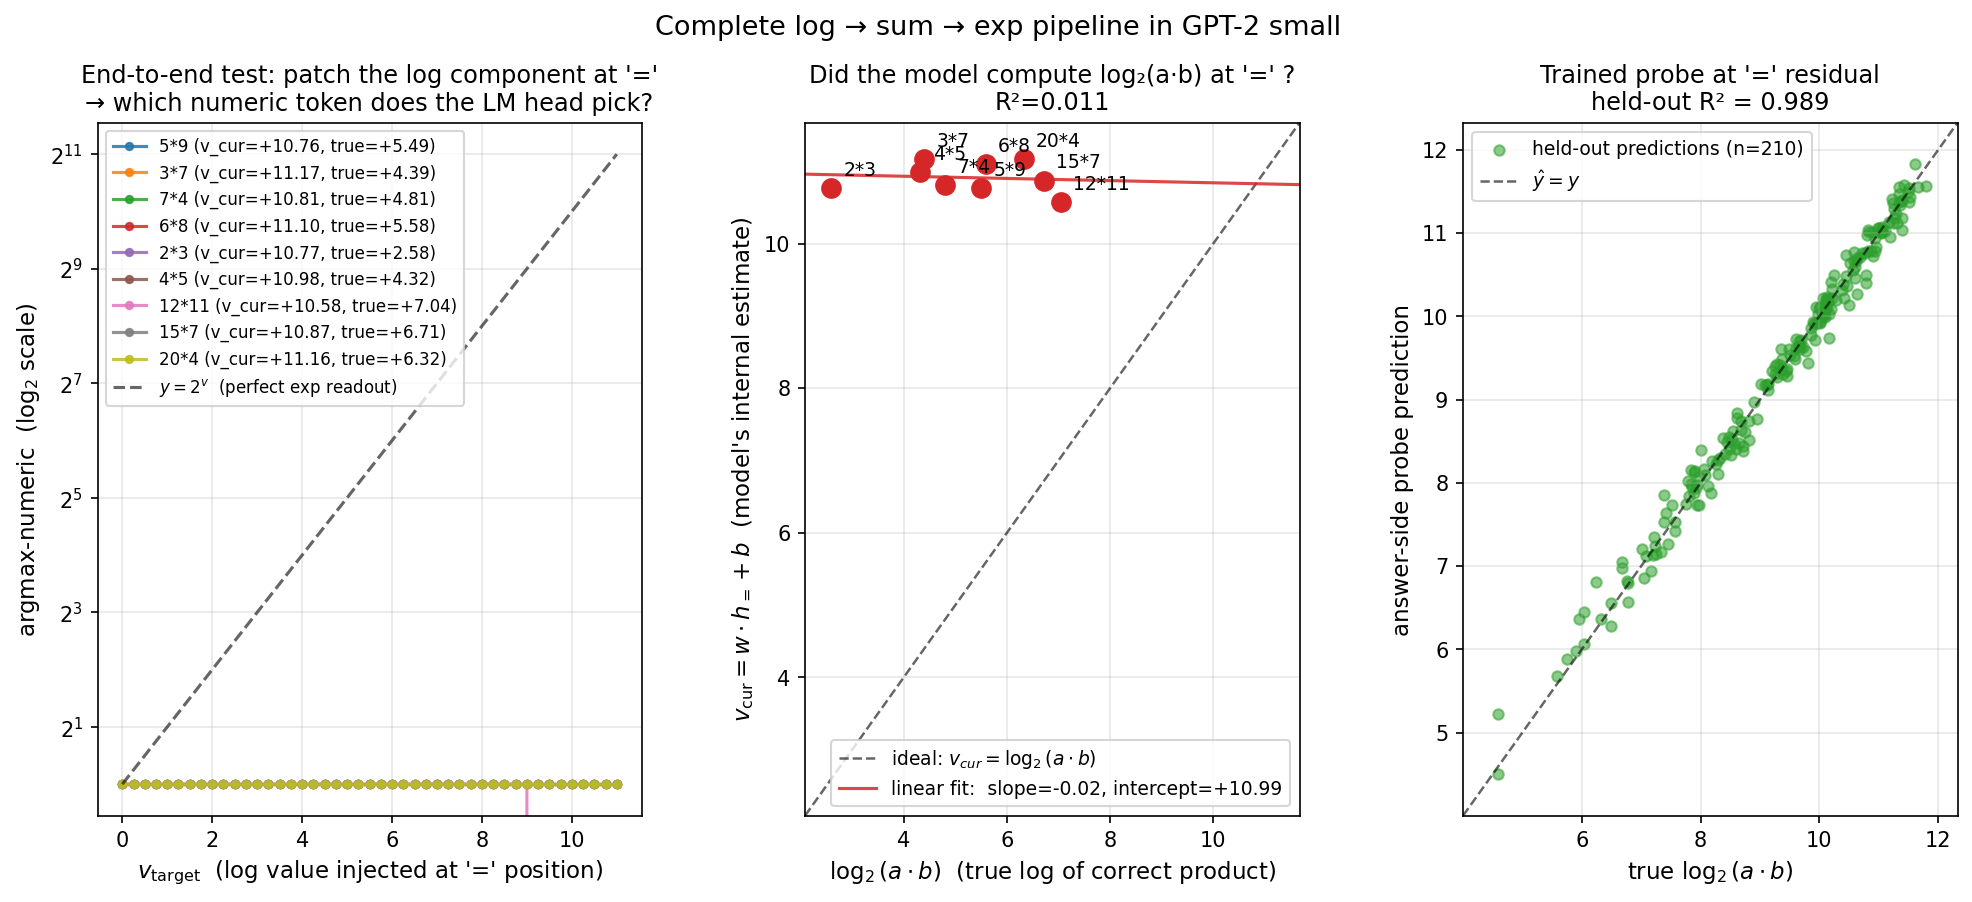
\includegraphics[keepaspectratio]{./probe_gpt2_pipeline.png}}

}

\caption{\label{fig-pipeline}The end-to-end pipeline. \textbf{Left:}
patching the log component at the \texttt{=} position of real prompts;
argmax-numeric is mostly stuck at \texttt{"\ 1"} regardless of
\(v_{\mathrm{target}}\). \textbf{Middle:} the operand-side probe's
readout at \texttt{=} is roughly constant (\textasciitilde10.8) across
all prompts, uncorrelated with \(\log_2(a \cdot b)\) (\(R^2 = 0.011\)).
\textbf{Right:} a fresh probe trained directly on residuals at
\texttt{=} predicts \(\log_2(a \cdot b)\) at \(R^2 = 0.989\) on held-out
pairs.}

\end{figure}%

\subsection{Why doesn't this give correct
arithmetic?}\label{sec-why-not-arithmetic}

Given that the circuit exists, why can't GPT-2 small actually multiply
\(5 \times 9\) and produce \(45\)? Across every prompt I tried, the
unpatched argmax over numeric tokens was \texttt{"\ 1"} or
\texttt{"\ 0"} --- the most generic possible guesses.

The answer is in the LM-head decomposition. The log axis captures 3.6\%
of each numeric row's squared norm. The other \textasciitilde96\% is
doing something --- most likely encoding general features like ``this is
a small number'', ``this is a common token'', and \(n\)-specific
text-frequency information. When the model asks ``what's the most likely
next token after \texttt{5\ *\ 9\ =}'', the answer is dominated by that
frequency mass, which favours \texttt{"\ 1"}, \texttt{"\ 0"}, and other
extremely common tokens. The log axis, even at 28\(\times\) baseline, is
one signal fighting against a much larger frequency prior.

This is consistent with the asymmetry seen in the operand-side patching:
moving the model's predictions \emph{toward} small numbers (with the
prior) is much easier than moving them toward large numbers (against the
prior). The machine is built. It just isn't loud enough.

A model with stronger arithmetic ability --- Pythia-1.4B, Llama-3.2-1B
--- should have the same circuit but with a louder log signal in the LM
head, enough to overcome the frequency prior. That's the obvious
follow-up.

\subsection{What this collectively shows}\label{sec-synthesis}

Three claims, in increasing order of strength.

The embedding layer of GPT-2 small encodes integers on an axis whose
shape is approximately logarithmic in magnitude, along with separate
axes for parity and last digit. Number-theoretic properties not visible
in surface text (\(\bmod 7\), primality) do not get a coherent
representation. This isn't surprising --- others have observed
log-shaped number representations in language models --- but the
controls here (the power-law sweep, the shuffled baseline, the
non-monotone targets) make it a clean measurement.

Perturbations along the embedding's log axis have structured, specific
causal effect on the model's next-token predictions in multiplication
prompts. Random directions of the same magnitude do not. This rules out
the most natural ``probe is just finding a noise direction'' null
hypothesis. The asymmetry of the effect (downward patches work, upward
patches partly fail) is itself informative --- it points at the LM
head's frequency prior as the limiting factor.

Most importantly, GPT-2 small does compute \(\log_2(a \cdot b)\)
somewhere in its residual stream by the time it reaches the \texttt{=}
token, and that computation is linearly readable at \(R^2 = 0.989\). The
model uses \emph{different} directions at the operand position and at
the \texttt{=} position; there is a translation step somewhere in the
middle layers. This is, as far as I know, novel for a model this small
--- and the strongest evidence I have that the full
\(\log \to \mathrm{sum} \to \exp\) circuit is mechanistically present in
GPT-2.

\subsection{Caveats}\label{sec-caveats}

The \(R^2 \approx 0.95\) for log decodability at the embedding is a
property of the embedding matrix. Because GPT-2 ties its LM head to its
embedding, the alignment of the LM head with the log axis is partly
architectural rather than independently learned. A model with untied
weights (Llama, Pythia) would give a cleaner test of whether the log
axis is emergent in both encoding and decoding separately. I'd expect it
to be --- but the test isn't clean here.

The causal-patching results in Figure~\ref{fig-patching} are measured on
relative logits among candidate products, not on argmax. GPT-2 small
genuinely cannot do most multiplications. The relative-logit shifts are
real and direction-specific, but they ride on top of a fixed frequency
prior. A much stronger version of the same experiment would run on a
model that can actually multiply, where patching should flip the argmax
cleanly.

The fitted answer-side probe at the \texttt{=} position has
\(R^2 = 0.989\) on \((a, b) \in [2, 64]^2\) pairs. Whether the same
direction carries \(\log_2(a \cdot b)\) for much larger operands is
untested.

The middle layers --- where the translation from input-log axis to
output-log axis happens --- are a black box in this study. Path-patching
across (layer, position) pairs would identify the attention heads that
move log information from the operand positions to the \texttt{=}
position, and the layer at which the sum happens. I haven't done it.

\subsection{Next steps}\label{sec-next}

The \textbf{exponentiation cross-check} is the sharpest immediate test.
If the model uses the log axis compositionally, patching \(\log(a)\) by
\(\Delta\) in an \texttt{a\^{}b\ =} prompt should shift the output's log
by \(b \cdot \Delta\), not \(\Delta\). That's a direct quantitative
prediction the model either passes or fails. Same patching code,
different prompts.

Re-running everything on \textbf{Pythia-1.4B or Llama-3.2-1B} would (a)
decouple the embedding and LM head via untied weights, (b) give a model
that can actually multiply, making the argmax test meaningful, and (c)
provide a larger residual dimension in which the per-direction norm
fractions become more informative.

\textbf{Path-patching to identify the layer and heads} where the
log-axis translation happens is the natural mechanistic follow-up. The
infrastructure for it is already in the patching code here; it needs
adaptation for attention-head outputs rather than residual-stream
patches.

\textbf{Scaling the embedding probe across the Pythia family} (70M,
160M, 410M, 1.4B, 2.8B, 6.9B) would give a clean test of how log-axis
quality varies with model size. The capacity-squeeze hypothesis predicts
something non-monotone --- small models need the shortcut, medium ones
can memorise a lookup table, large ones can host both --- but any clean
trend would be informative.

\subsection{Code and data}\label{sec-code}

All scripts and figures are in the project folder.

{\def\LTcaptype{none} % do not increment counter
\begin{longtable}[]{@{}ll@{}}
\toprule\noalign{}
File & Produces \\
\midrule\noalign{}
\endhead
\bottomrule\noalign{}
\endlastfoot
\texttt{reasoning\_router.py} & Figure~\ref{fig-toy-routing} \\
\texttt{probe\_gpt2\_log.py} & per-layer probe (precursor to
Figure~\ref{fig-controls}) \\
\texttt{probe\_gpt2\_controls.py} & Figure~\ref{fig-controls} +
power-law sweep \\
\texttt{probe\_gpt2\_patching.py} & Figure~\ref{fig-patching} \\
\texttt{probe\_gpt2\_lmhead.py} & Figure~\ref{fig-lmhead} \\
\texttt{probe\_gpt2\_pipeline.py} & Figure~\ref{fig-pipeline} + the
answer-side probe \\
\end{longtable}
}

All scripts are self-contained Python and reproduce on CPU in about ten
minutes total. GPT-2 small downloads at \textasciitilde500 MB.
Dependencies: \texttt{torch}, \texttt{transformers},
\texttt{scikit-learn}, \texttt{matplotlib}.

\begin{center}\rule{0.5\linewidth}{0.5pt}\end{center}

\begin{tcolorbox}[enhanced jigsaw, arc=.35mm, bottomrule=.15mm, bottomtitle=1mm, breakable, colback=white, colbacktitle=quarto-callout-tip-color!10!white, colframe=quarto-callout-tip-color-frame, coltitle=black, left=2mm, leftrule=.75mm, opacityback=0, opacitybacktitle=0.6, rightrule=.15mm, title=\textcolor{quarto-callout-tip-color}{\faLightbulb}\hspace{0.5em}{Methodological takeaway}, titlerule=0mm, toprule=.15mm, toptitle=1mm]

Probes are cheap. If a probe trained in position A gives no signal in
position B, that doesn't mean the information isn't in B --- it might
just mean B uses a different direction. Fit a fresh probe at the
position you actually care about before concluding the circuit is
absent. In this study, that one habit was the difference between ``no
circuit found'' and ``circuit found at \(R^2 = 0.989\)''.

\end{tcolorbox}

\emph{Thanks to the rough plan in \texttt{experiment1.md} for the
framing. The mechanistic-interpretability moves (linear probing,
activation patching) are standard tools from the literature; what this
post adds is the specific finding that GPT-2 small computes
\(\log_2(a \cdot b)\) on a different axis than the one it uses to read
operand magnitudes.}




\end{document}
